\section{Gearing}
I \cref{sensorer:motorer} fandt vi ud af at præcisionen på motorerne ikke var høj.
Der var en afvigelse på op til 4\dg, imod en forventet afvigelse på 1\dg.
Selv hvis den forventede afvigelse kunne blive overholdt, kan denne stadig give for stor usikkerhed.

\subsection{Gearing af motorer}
For at sænke denne upræcision vil der blive indført gearing.
Dette er især vigtigt for den motor der roterer den ultrasoniske sensor, men også for de motorer som driver hjulene.

\paragraph{Den ultrasoniske sensor} bruges til at bestemme tilkendegivelse og afstand af et objekt i en bestemt retning, derfor vil det være en klar fordel jo højere sikkerhed og præcision der kan opnås når denne retning skal bestemmes.

\paragraph{Hjulene} har vist problemer med at holde fat i underlaget, derfor vil det være en fordel at geare så der kan opnås et højere moment.
Igen er tid ikke en faktor, så det er acceptabelt at robotten mister fart.
Præcision af motorernes position er heller ikke vigtig, da lokationen bestemmes andetsteds og ikke vha. \textit{dead reckoning}.

\subsection{Simpel Teori}
Gearing kan foregå på to måder; geare op eller geare ned.
Det gear der er knyttet direkte til motoren kalder vi fører-gearet og det gear der er knyttet til fører-gearet kalder vi for følger-gearet.
Eksempel på nedgearing, som er det eneste vi kommer til at bruge:

\begin{figure}[H]
\centering

\includegraphics[width=.5\textwidth]{gears/op_og_ned}
\end{figure}

\subsubsection{Nedgearing}
Nedgearing foregår ved at et mindre gear driver et større gear.
Ratio'en (størrelsen af gearing) er styret af antallet af tænder på gearene.
For eksempel vil et 24-tands fører-gear drive et 40-tands følger-gear med ratio'en $\frac{40}{24}$, hvilket betyder at der går 40 fører omdrejninger pr. 24 følger omdrejninger. Dvs. at motoren der driver fører-gearet skal rotere $\frac{40}{24} = 1 \frac{2}{3}$ omgange for at rotere følger-gearet én omgang.

\subsection{Vores gearing}
Her vil blive forklaret den teoretiske gearing for henholdsvis ultrasonisk sensor og hjul.

\subsubsection{Ultrasonisk sensor}
Gearingen for den ultrasoniske sensor består af i alt 4 tandhjul, som alle kan ses i \cref{gearing:tandhjul}.

Den første kombination består af en orm som fører-gear og 40-tands som følger-gear.
Ormen kræver en hel rotation for at flytte én tand.
Dette giver ratio'en $\frac{40}{1} = 40$, dvs. at der kræves 40 hele rotationer med motoren for at rotere 40-tands gearet én omgang.

Den anden kombination består af en 24-tands som fører-gear og en 56-tands som følger-gear.
Dette giver ratio'en $\frac{56}{24} = 2 \frac{1}{3}$.

Den samlede rotation er således: $$40 \cdot 2\frac{1}{3} = 93 \frac{1}{3}$$.

\subsubsection{Hjul}
Gearingen for hjulene består hver især af to tandhjul; ét 40-tands og ét 24-tands.
Derved er gearingen som i det eksemplet: $$ \frac{40}{24} = 1 \frac{2}{3} $$

\subsection{Test af gearing}
Nu hvor den teoretiske gearing er fastlagt, vil der her blive udført forsøg for at afgøre præcisionen af motorerne med gearing, evt. at fastlægge en faktisk gearing, hvis denne afviger fra den teoretiske.

\begin{figure}[h]
\centering
\begin{subfigure}[b]{.2\textwidth}

\includegraphics[width=\textwidth]{gears/24-tooth}
\caption{24-tands}
\end{subfigure}
\begin{subfigure}[b]{.2\textwidth}
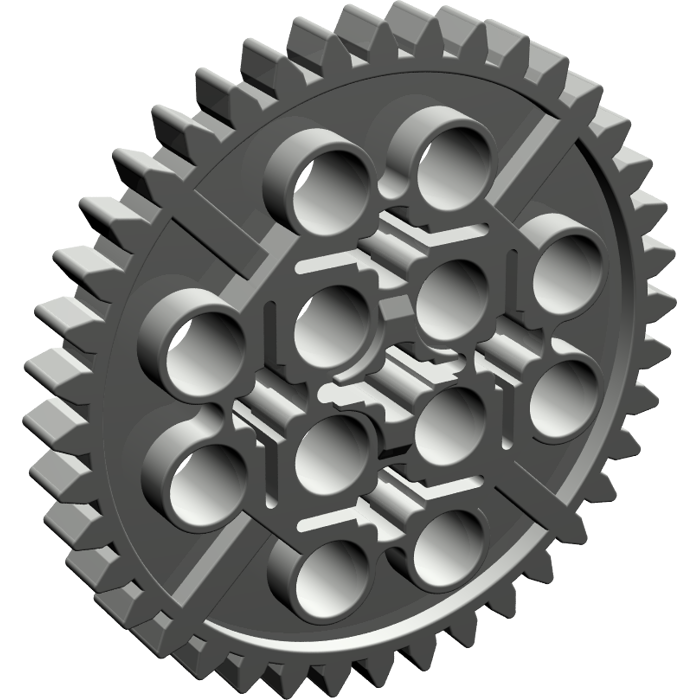
\includegraphics[width=\textwidth]{gears/40-tooth}
\caption{40-tands}
\end{subfigure}
\begin{subfigure}[b]{.2\textwidth}
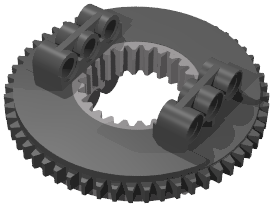
\includegraphics[width=\textwidth]{gears/turntable}
\caption{56-tands \\ \centering (drejeskive)}
\end{subfigure}
\begin{subfigure}[b]{.2\textwidth}
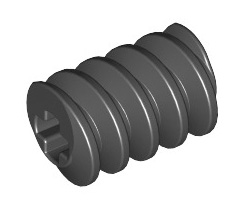
\includegraphics[width=\textwidth]{gears/worm}
\caption{Orm}
\end{subfigure}
\caption{De anvendte tandhjul}
\label{gearing:tandhjul}
\end{figure}